\documentclass{beamer}[10]
\usepackage{pgf}
\usepackage[portuguese]{babel}
\usepackage[utf8]{inputenc}
\usepackage{beamerthemesplit}
\usepackage{graphics,epsfig,subfigure}
\usepackage{url}
\usepackage{srcltx}
\usepackage{hyperref}

\definecolor{kugreen}{RGB}{50,93,61}
\definecolor{kugreenlys}{RGB}{132,158,139}
\definecolor{kugreenlyslys}{RGB}{173,190,177}
\definecolor{kugreenlyslyslys}{RGB}{214,223,216}
\setbeamercovered{transparent}
\mode<presentation>
\usetheme[numbers,totalnumber,compress,sidebarshades]{PaloAlto}
\setbeamertemplate{footline}[frame number]

  \usecolortheme[named=kugreen]{structure}
  \useinnertheme{circles}
  \usefonttheme[onlymath]{serif}
  \setbeamercovered{transparent}
  \setbeamertemplate{blocks}[rounded][shadow=true]

\logo{
\includegraphics[width=1.2 cm]{unb_0}}
%\useoutertheme{infolines} 
\title{Estudo de barreiras para contribuir com projetos de software público brasileiro}
\author[]{Camila Ferreira Pereira Silva \\ Orientador:  Prof. Dr. Paulo Roberto Miranda Meirelles}
\institute{Faculdade UnB Gama \\ Universidade de Brasília}
\date{2 de dezembro de 2016}


\begin{document}

\frame{
\titlepage \vspace{1cm}
}

\frame
{
\frametitle{Agenda}
\tableofcontents%[pausesection]
}

\section{Introdução}

\frame{
\frametitle{Introdução}
\begin{itemize}
\item O surgimento da internet possibilitou novas formas de colaboração e desenvolvimento de software.
\item Mas não derrubou todas as barreiras.
	\begin{itemize}
	\item Falta de conhecimento técnico;
	\item Desenvoltura social.
	\end{itemize}
\item Pesquisa do professor Igor Steinmancher tem o propósito de investigar essas barreiras.
\item Software público nasceu com o objetivo de economizar recursos pelo governo brasileiro.
\end{itemize}
}

\frame{
\frametitle{Objetivos}
Os objetivos específicos desse trabalho são:
\begin{itemize}
\item Analisar e entender as barreiras enfrentadas pelos desenvolvedores ao começar
a contribuir com um projeto de software livre de acordo com a pesquisa do professor Igor Steinmancher;
\item Mapear as barreiras enfrentadas pelos desenvolvedores ao começar a contribuir
com um projeto de software público;
\item Comparar as barreiras encontradas para projetos de software público com as 
barreiras já conhecidas para começar 
a contribuir com projetos de sofware livre;
\item Iniciar o desenvolvimento de uma nova versão do portal FlossCoach.
\end{itemize}

}

\section{Software Livre}

\frame{
\frametitle{Software Livre}
\begin{itemize}
\item Desde o início da computação a maior parte dos desenvolvedores 
trabalhava da forma que hoje identificamos como software livre.
\item Alicerce na liberdade do usuário.
\item Segue o estilo Linus Trovalds de desenvolvimento, libere cedo e frequentemente.
\item As liberdades e garantias sobre o software são estabelecidas 
no Brasil pela lei de direitos autorais.
\end{itemize}
}

\frame{
\frametitle{Lei de Direitos Autorais}
\begin{itemize}
\item A legislação brasileira vê o software menos como produto e mais como expressão intelectual.
\item (Lei 9609/98 e Lei 9279/98, art. 10)
\item Cabe ao titular do direito autoral a definição da forma como disporá desse direito.
\end{itemize}
}

\frame{
\frametitle{Licenças de software}
\begin{itemize}
\item A maioria dos produtos de software utilizam licenças restritivas.
\item Para que um software seja dito livre precisa ter um desses tipos de licenças:
	\begin{itemize}
	\item Permissivas(BSD, MIT/X11 e Apache);
	\item Recíprocas totais(GPL);
	\item Recíprocas parciais(LGPL e Licença Mozilla).
	\end{itemize}
\end{itemize}
}


\frame{
\frametitle{Portal do Software Público Brasileiro}
\begin{itemize}
\item Sistema web que se consolidou como ambiente de compartilhamento de software.
\item Propósito inical era de que fosse apenas para uso do governo.
\item Característica de bem público ao software.
\item Instrução Normativa 04/2012.
\item A antiga versão ficou obsoleta por não acompanhar a evolução de seu framework OpenACS.
\end{itemize}
}

\frame{
\frametitle{Novo Portal SPB}
Desenvolvido pela Universidade de Brasília,
através dos seus Laboratórios LAPPIS e MídiaLab em parceria com o Centro de
Competência em Software Livre da Universidade de São Paulo(CCSL-USP).
\begin{figure}[h]
	\centering
	\label{arquitetura}
		\includegraphics[keepaspectratio=true,scale=0.15]{figuras/arquitetura.eps}
	\caption{Arquitetura do novo SPB}
\end{figure}
}

\frame{
\frametitle{Novo Portal SPB}
\begin{itemize}
\item Portaria N o 46, de 28 de Setembro de 2016.
	\begin{itemize}
	\item Definição dos papéis dos envolvidos no SPB.
	\item Criação de novos tipos de comunidade dentro da plataforma.
	\item Flexibilização das licenças que podem ser aplicadas a software público.
	\item Não mais obrigatoriedade do registro no INPI.
	\end{itemize}
\item Portaria N o 48, de 28 de Setembro de 2016.
	\begin{itemize}
	\item Atualização anual das informações no Portal do SISP.
	\end{itemize}
\end{itemize}
}

\section{Barreiras para contribuir com software livre}

\frame{
\frametitle{Barreiras para contribuir com software livre}
\begin{itemize}
\item Pesquisa de doutorado do professor Igor Steinmancher.
\item Objetivo de encontrar barreiras enfrentadas por novos desenvolvedores
para começar a contribuir com projetos de software livre.
\item Análise qualitativa feita com estudantes de diferentes projetos de software livre.
\item Utilizando questionários e entrevistas.
\end{itemize}
}

\frame{
\frametitle{Barreiras para contribuir com software livre}
A análise dos dados dos questionários e entrevistas foi feito com base na \textit{Ground Theory}. 
\begin{enumerate}
\item Codificação aberta;
\item Codificação axial;
\item Seleção de código.
\end{enumerate}
}

\frame{
\frametitle{Barreiras para contribuir com software livre}
Após as análises dos questionários foram encontradas 58 barreiras, divididas em 6 categorias:
\begin{itemize}
\item Tarefas de recepção de novos contribuidores;
\item Características dos novos contribuidores;
\item Orientação aos novos contribuidores;
\item Diferenças culturais;
\item Problemas na documentação;
\item Dificuldades técnicas.
\end{itemize} 
}

\frame{
\frametitle{Barreiras para contribuir com software livre}
Modelo encontrado pela análise dos questionários e entrevistas.
\begin{figure}[h]
	\centering
	\label{barreiras}
		\includegraphics[keepaspectratio=true,scale=0.1]{figuras/Barreiras.eps}
	\caption{Barreiras para contribuir com Software livre.}
\end{figure}
}


\frame{
\frametitle{O portal para suporte a novos contribuidores: FLOSSCoach}
\begin{figure}[h]
	\centering
	\label{flosscoach}
		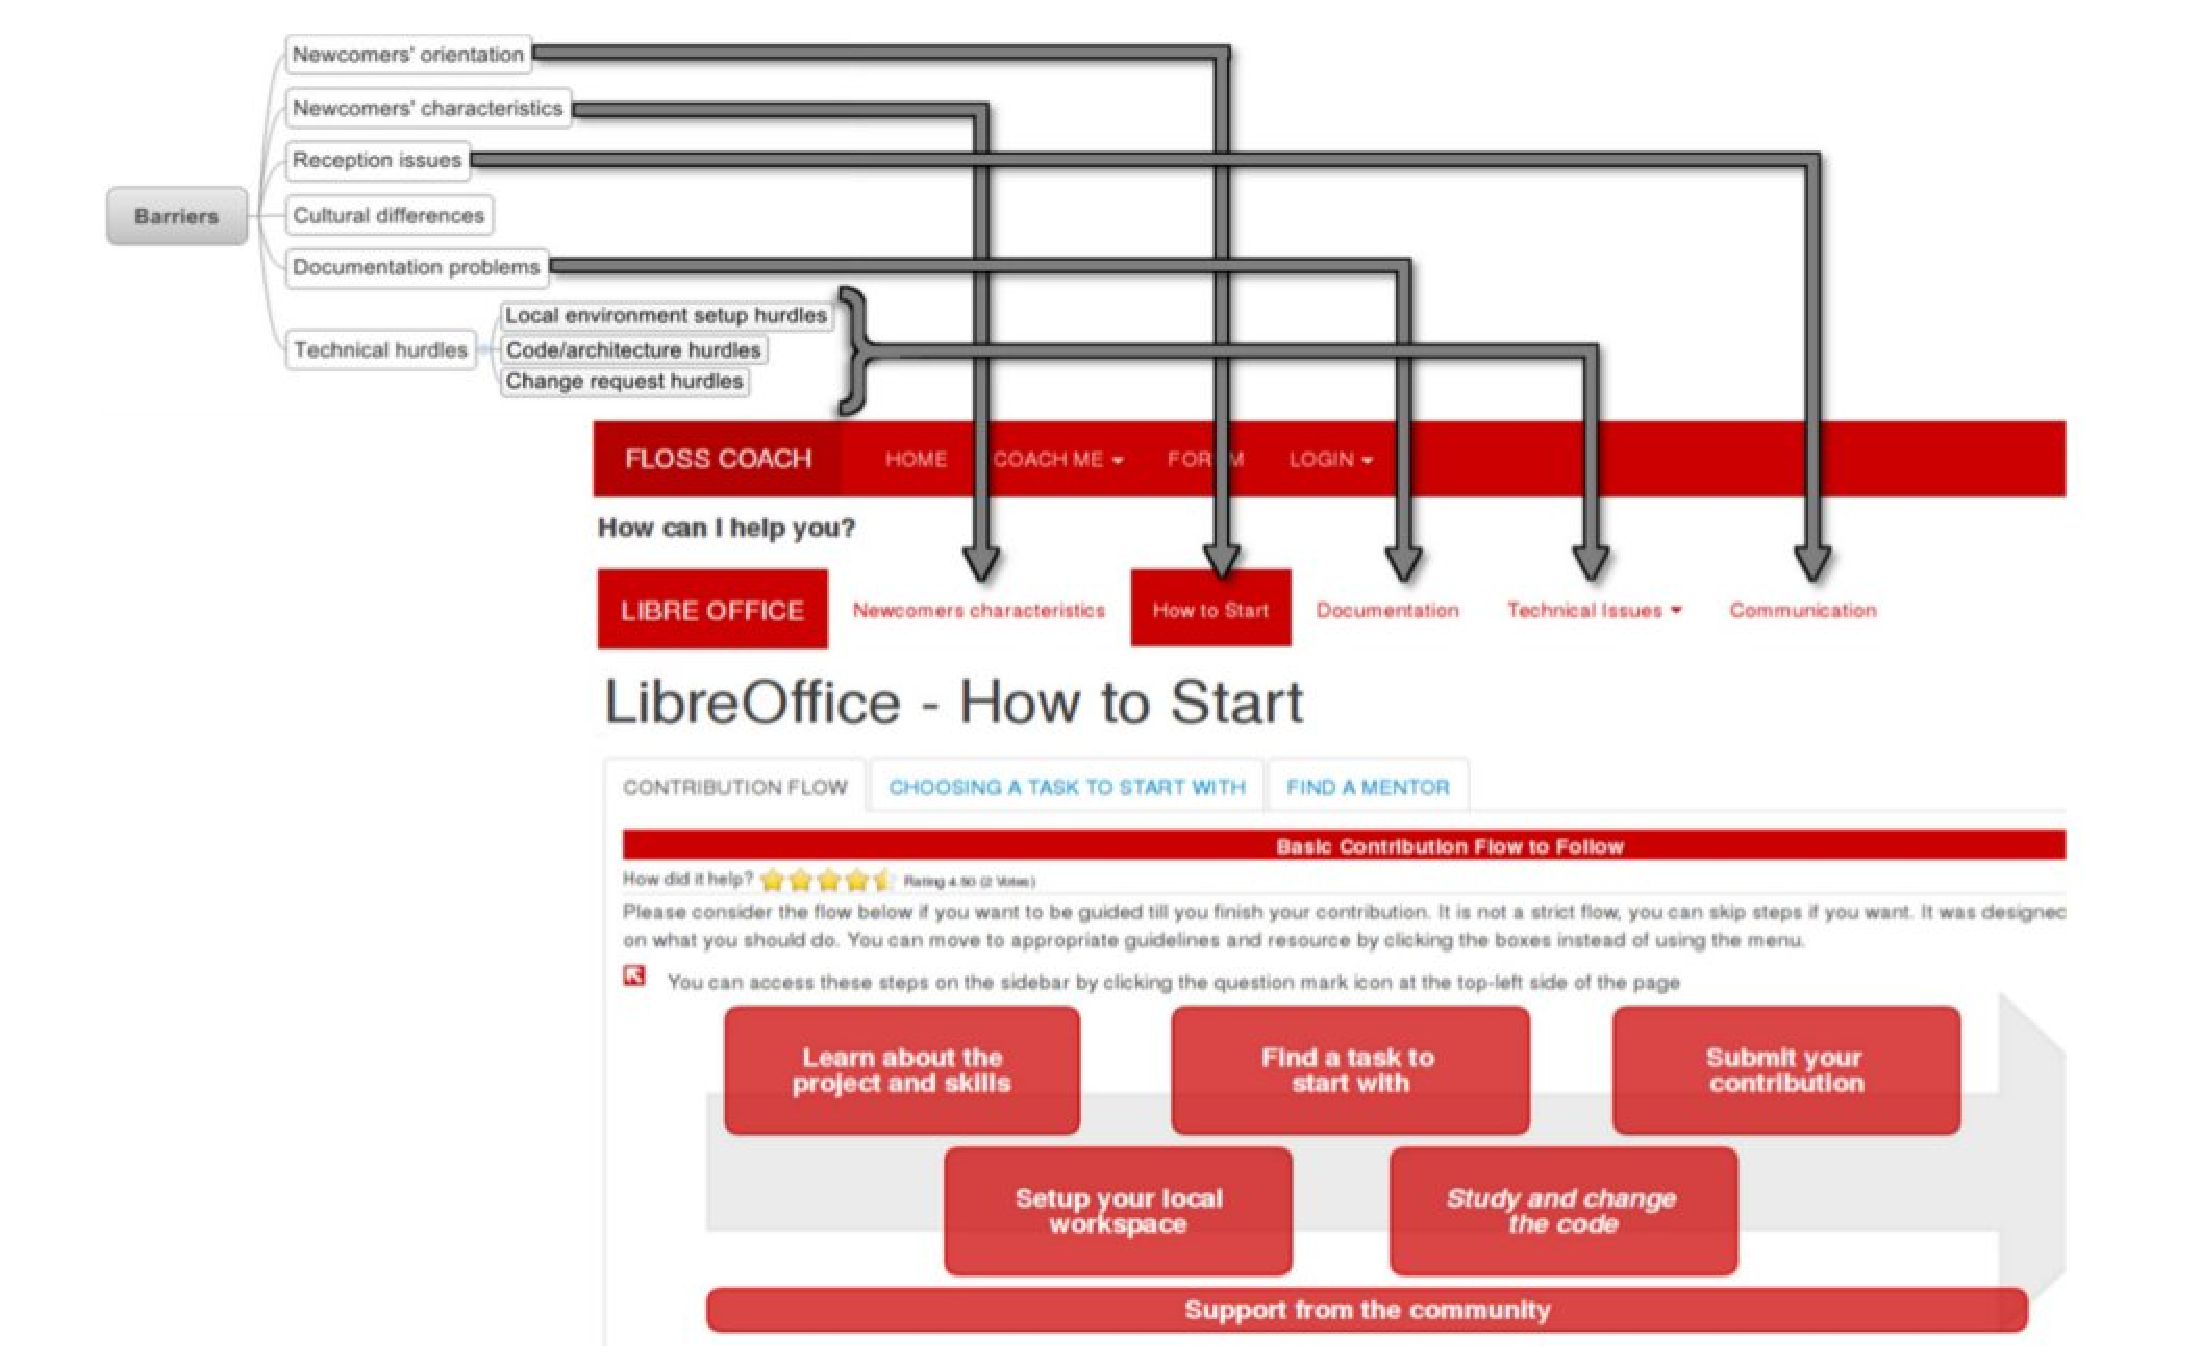
\includegraphics[keepaspectratio=true,scale=0.2]{figuras/portal.eps}
	\caption{Portal para suporte a novos contribuidores.}
\end{figure}
}

\frame{
\frametitle{O portal para suporte a novos contribuidores: FLOSSCoach}
Cada categoria passou a ser uma aba dentro do portal:
\begin{itemize}
\item How to Start - Orientações a novos contribuidores;
\item Newcomers’ characteristics - Comportamento dos novos contribuidores;
\item Communication - Interação dos novos contribuidores;
\item Documentation - Documentos do projeto;
\item Technical issues - Dificuldades técnicas dos novos contribuidores.
\end{itemize}

Esta primeira versão do FlossCoach era estática.
\\Baseada em Joomla.
}

\section{Metodologia}

\frame{
\frametitle{Metodologia}
\begin{itemize}
\item O Software Livre possui um mecanismo de produção colaborativo e dinâmico.
\item O sucesso de um projeto de software livre depende fortemente de um grande 
número de desenvolvedores colaborando em rede.
\item Motivo de que o processo de entrada de novos desenvolvedores nas comunidades merece atençao.
\item Software público enfrenta os mesmos desafios.
\item O modelo típico do software livre se diferencia em muitos aspectos com a forma que
o governo brasileiro desenvolve software. 
\end{itemize}
}

\frame{
\frametitle{Metodologia}
\begin{block}{Questão de Pesquisa}
Existem mais barreiras para começar a contribuir com um projeto de software
público do que com um projeto de software livre?
\end{block}
}

\frame{
\frametitle{Metodologia}
\begin{itemize}
\item Replicamos a pesquisa de doutorado do professor Igor Steinmancher.
\item Escolhemos 6 comunidades do portal SPB:
	\begin{itemize}
	\item Noosfero;
	\item Cacic;
	\item SAE - Sistema de apoio educacional;
	\item I-Educar;
	\item E-Sic;
	\item SEI - Sistema Eletrônico de informações.
	\end{itemize}
\item Enviamos os questionários adaptados a essas comunidades e aos seus coordenadores.
\end{itemize}
}

\frame{
\frametitle{Metodologia de desenvolvimento}
O desenvolvimento do novo Portal FlossCoach foi dividido em 3 fases:
	\begin{enumerate}
	\item Desenvolvimento do protótipo Funcional;
	\item Desenvolvimento pela equipe de bolsistas;
	\item Desenvolvimento paralelo dos bolsistas e alunos da disciplina de Manutenção e
Evolução de Software.
	\end{enumerate}

}

\frame{
\frametitle{Metodologia de desenvolvimento}
Nossos papéis também foram diferentes nas 3 fases do desenvolvimento.
\begin{enumerate}
\item Desenvolvedores;
\item Arquitetos de software;
\item Desenvolvedores, Arquitetos de software e \textit{Product Owner} na disciplina de MES.
\end{enumerate}
}

\section{Barreiras para contribuir com software público}

\frame{
\frametitle{Barreiras para contribuir com software público}
\begin{itemize}
\item Para levantar as barreiras enviamos os questionários às comunidades e os deixamos disponíveis por 2 meses.
\item Obtivemos 19 respostas de desenvolvedores e 3 respostas de coordenadores.
\item 90\% dos desenvolvedores e 100\% dos coordenadores estavam em seu primeiro projeto de software público.
\item 40\% dos desenvolvedores eram pagos para desenvolver software público.
\item 40\% dos desenvolvedores tinha o desenvolvimento de software público como sua principal ocupação.
\end{itemize}
}

\frame{
\frametitle{Barreiras para contribuir com software público}
\begin{itemize}
\item Os conceitos foram extraídos conforme apareciam nas respostas dos questionários, de acordo com a primeira etapa da \textit{Ground Theory}.
\item Algumas questões se sobressairam com relação a semelhança nas respostas, por exemplo.
\end{itemize}
\begin{block}{Questão do questionário}
``Qual era o seu conhecimento em software público 
quando você iniciou no projeto?''
\end{block}

\begin{itemize}
\item Em 18 das 19 respostas os desenvolvedores responderam que era básico, nenhum ou pouco.
\item Dessas respostas nós conseguimos, com certeza,
afirmar que a “Falta de conhecimento em software público” é uma barreira.
\end{itemize}
}

\frame{
\frametitle{Barreiras para contribuir com software público}
\begin{itemize}
\item Dessa forma chegamos a uma lista inicial de 62 barreiras.
\item Após a aplicação da segunda e terceira fases da \textit{Ground Theory} chegamos a 50 barreiras divididas em 6 categorias.
	\begin{itemize}
	\item Conhecimento em software livre e público;
	\item Hierarquia;
	\item Orientação a novos desenvolvedores;
	\item Documentação;
	\item Dificuldades técnicas;
	\item Características dos novos contribuidores.
	\end{itemize} 
\end{itemize}
}

\frame{
\frametitle{Barreiras para contribuir com software público}
\begin{figure}[h]
	\centering
	\label{fig:SPbarreiras}
		\includegraphics[keepaspectratio=true,scale=0.12]{figuras/Barreiras_Software_Publico_.eps}
	\caption{Barreiras para contribuir com projetos de software público.}
\end{figure}
}

\frame{
\frametitle{Análise comparativa com as barreiras conhecidas de Software Livre}
Barreiras apenas para software livre.
\begin{figure}[h]
	\centering
	\label{fig:barreiras}
		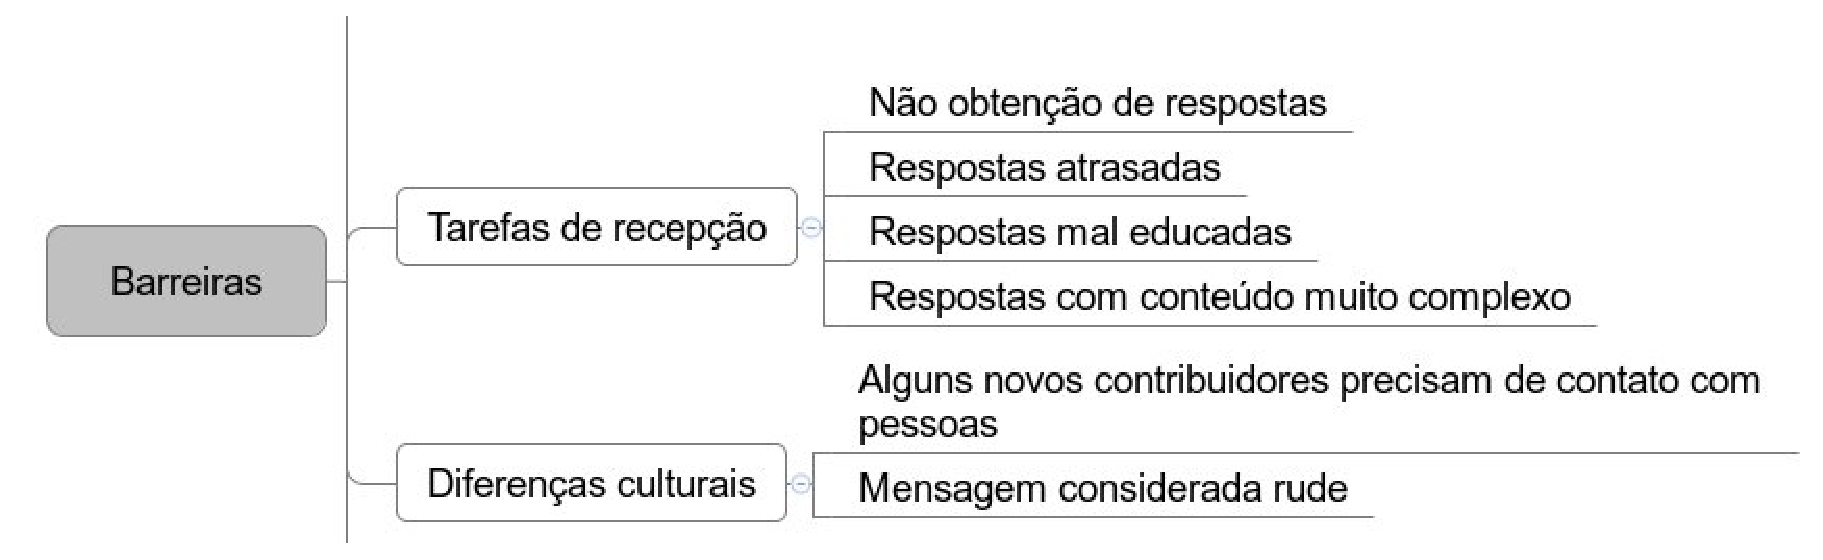
\includegraphics[keepaspectratio=true,scale=0.3]{figuras/barreirassoSL.eps}
	\caption{Categorias Tarefas de Recepçao e Diferenças Culturais.}
\end{figure}

}

\frame{
\frametitle{Análise comparativa com as barreiras conhecidas de Software Livre}
Barreiras apenas para software público.
\begin{figure}[h]
	\centering
	\label{fig:conhecimentos}
		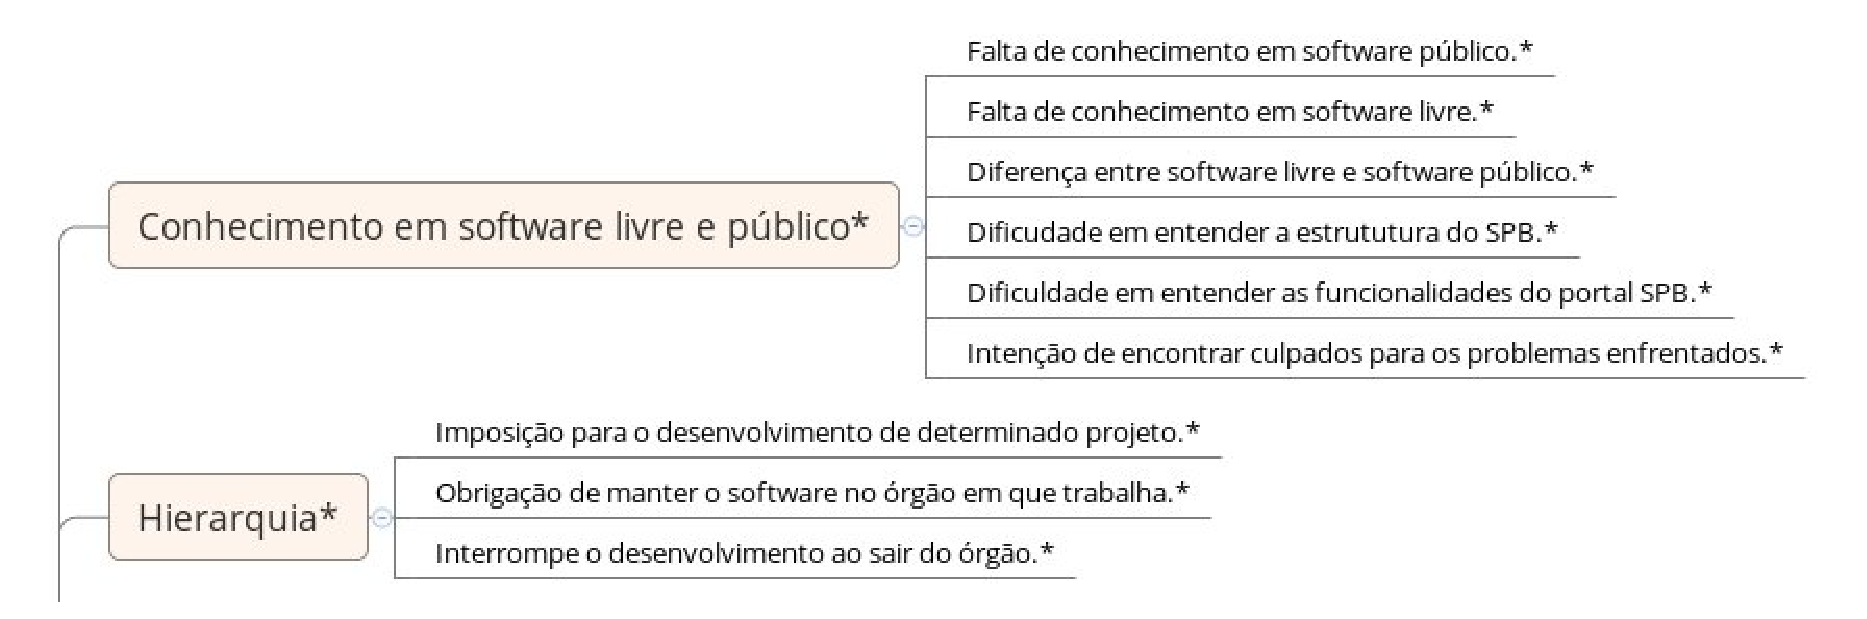
\includegraphics[keepaspectratio=true,scale=0.3]{figuras/conhecimentos.eps}
	\caption{Categorias Conhecimentos e Hierarquia.}
\end{figure}
}

\frame{
\frametitle{Análise comparativa com as barreiras conhecidas de Software Livre}
Barreiras tanto para projetos de software público quanto para projetos de software livre.
\\Com execessão das motivações financeira e social.
\begin{figure}[h]
	\centering
	\label{fig:caracteristicas}
		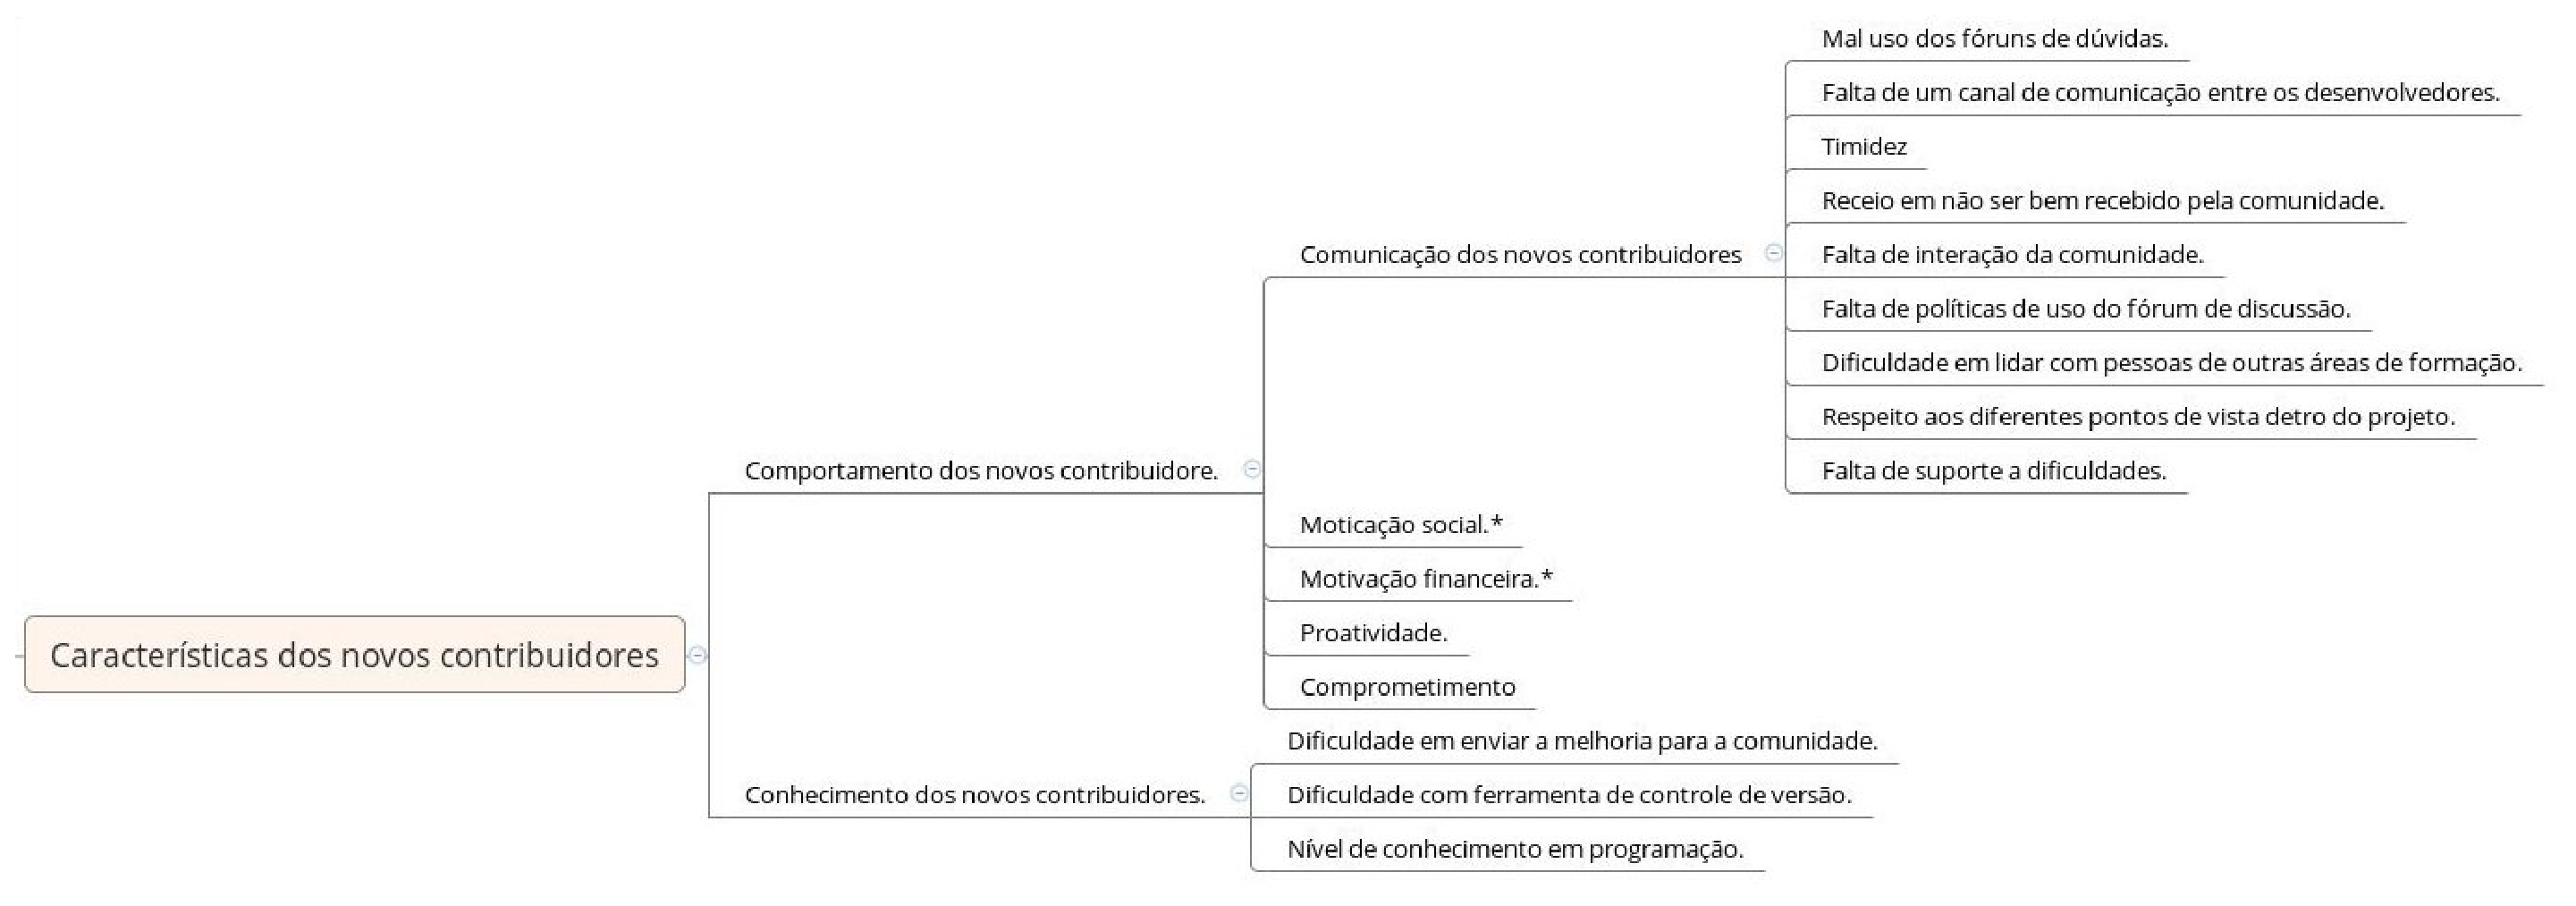
\includegraphics[keepaspectratio=true,scale=0.2]{figuras/caracteristicas.eps}
	\caption{Categoria Características dos novos contribuidores.}
\end{figure}
}

\frame{
\frametitle{Análise comparativa com as barreiras conhecidas de Software Livre}
Barreiras tanto para projetos de software público quanto para projetos de software livre.
\begin{figure}[h]
	\centering
	\label{fig:documentacao}
		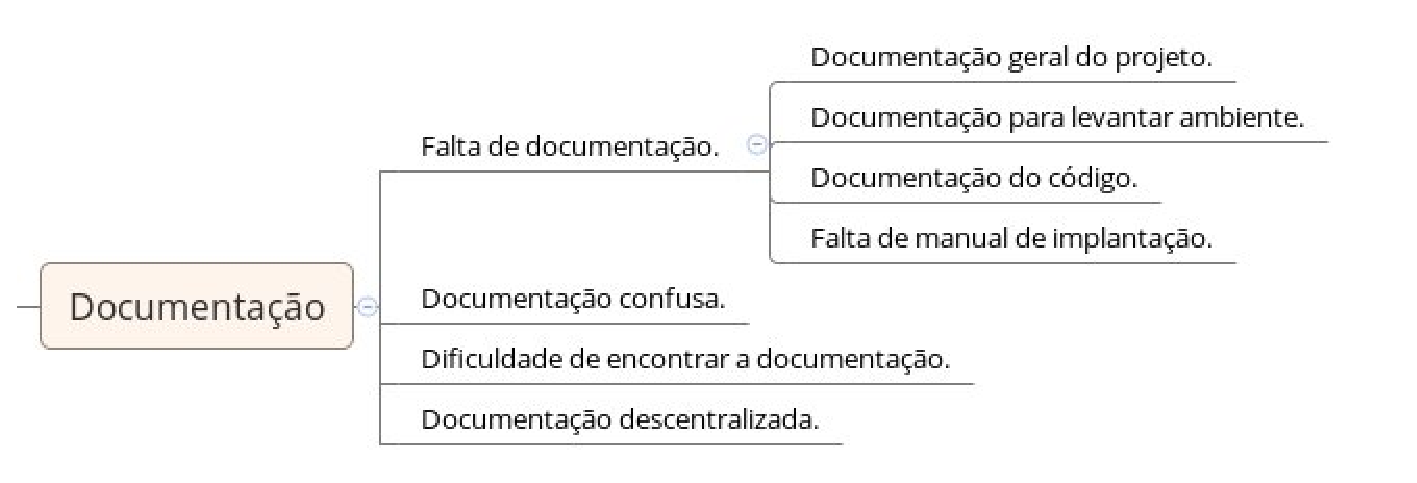
\includegraphics[keepaspectratio=true,scale=0.3]{figuras/documentacao.eps}
	\caption{Categoria Documentação.}
\end{figure}
}

\frame{
\frametitle{Análise comparativa com as barreiras conhecidas de Software Livre}
Barreiras tanto para projetos de software público quanto para projetos de software livre.
\\Para software público é ainda mais grave, quando fazemos uma ligação com as Características dos novos contribuidores.
\begin{figure}[h]
	\centering
	\label{fig:dificuldades}
		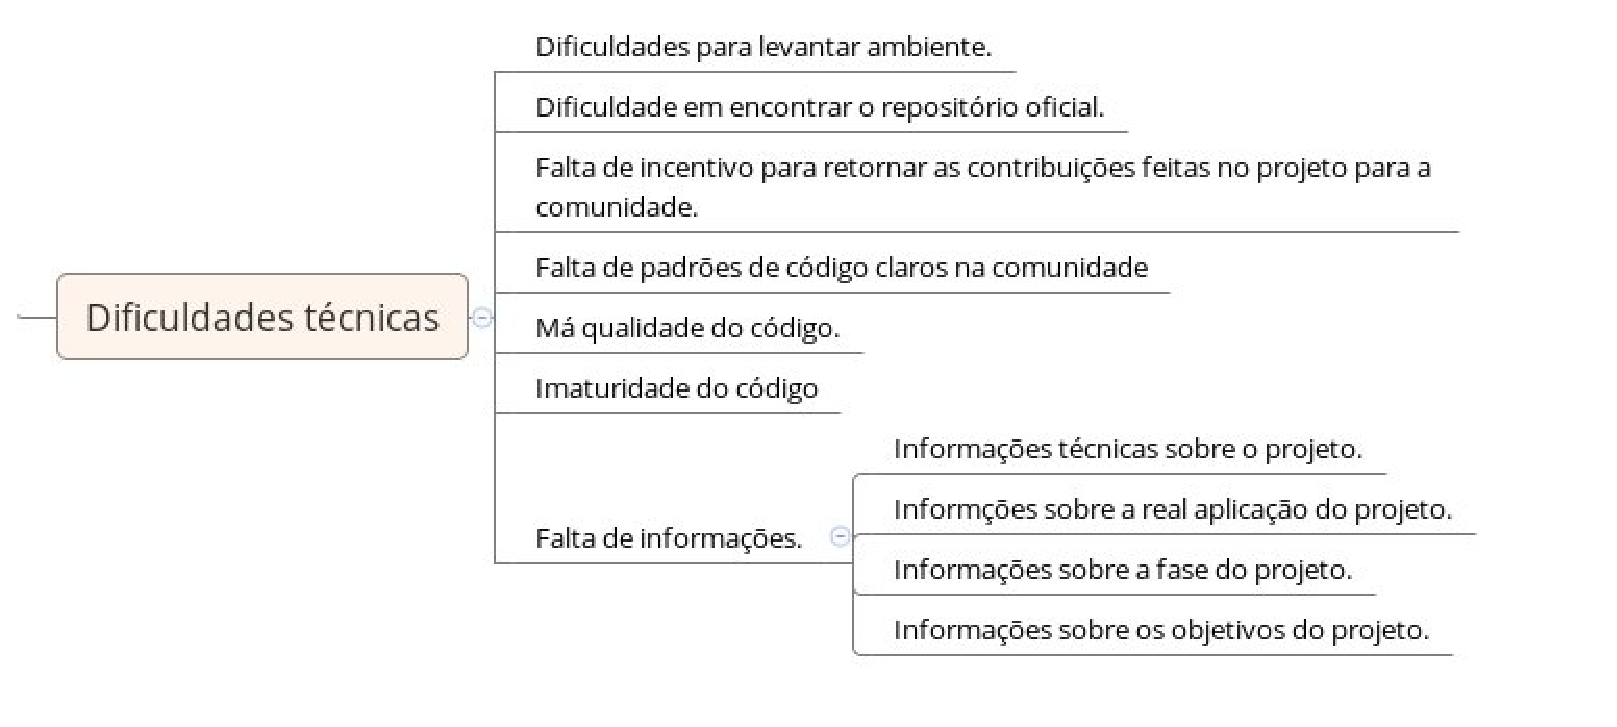
\includegraphics[keepaspectratio=true,scale=0.3]{figuras/dificuldades.eps}
	\caption{Categoria Dificuldades Técnicas.}
\end{figure}
}

\frame{
\frametitle{Análise comparativa com as barreiras conhecidas de Software Livre}
Barreiras tanto para projetos de software público quanto para projetos de software livre.
\begin{figure}[h]
	\centering
	\label{fig:orientacoes}
		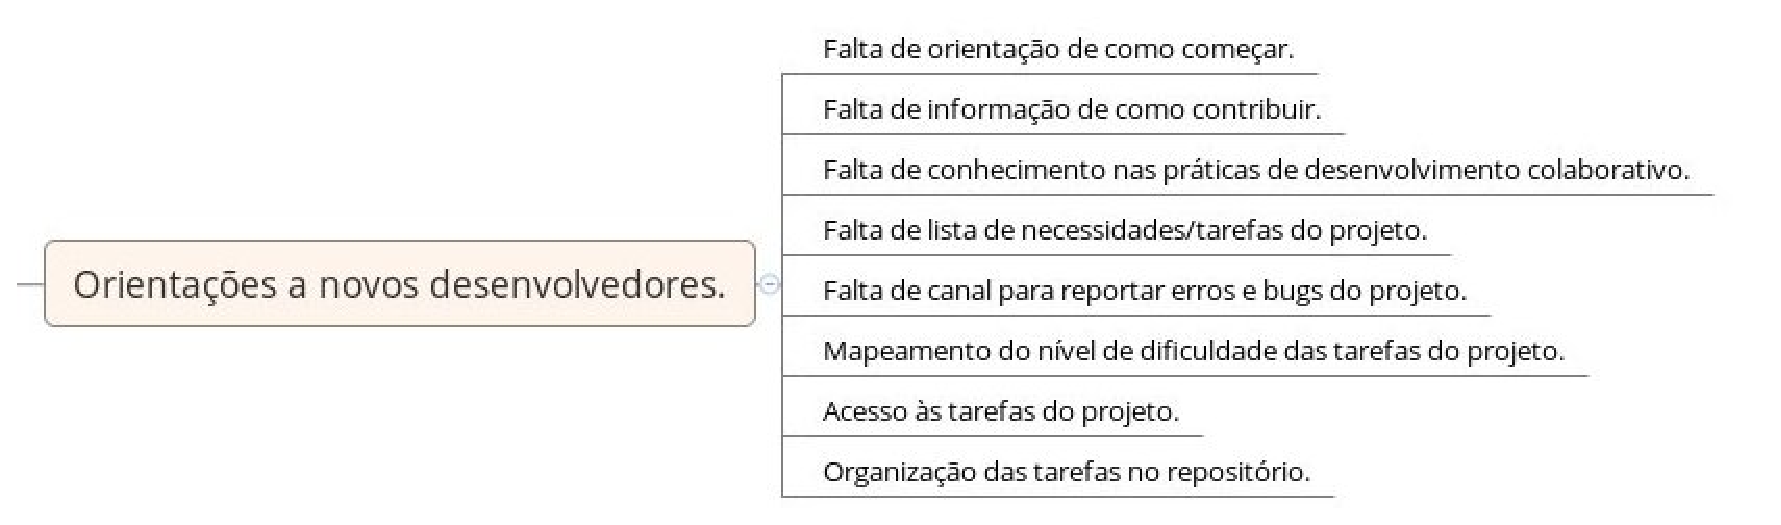
\includegraphics[keepaspectratio=true,scale=0.3]{figuras/orientacoes.eps}
	\caption{Categoria Orientações a novos contribuidores.}
\end{figure}
}

\section{Desenvolvimento}
\frame{
\frametitle{Desenvolvimento do novo Portal FlossCoach}
\begin{itemize}
\item O desenvolvimento do novo Portal FlossCoach foi dividido em 3 fases.
\item O objetivo da primeira fase do desenvolvimento era que tivéssemos como cadastrar
os projetos com os campos para cadastro que já eram relatados no portal FlossCoach além
de um cadastro de usuários.
\item Foi desenvolvido em \textit{Ruby on Rails} e \textit{Bootstrap}.
\item Essa fase do desenvolvimento durou 4 meses, de dezembro de 2015 a março de 2016.
\end{itemize}
}

\frame{
\frametitle{Desenvolvimento do novo Portal FlossCoach}
\begin{figure}[h]
	\centering
	\label{fig:inicial}
		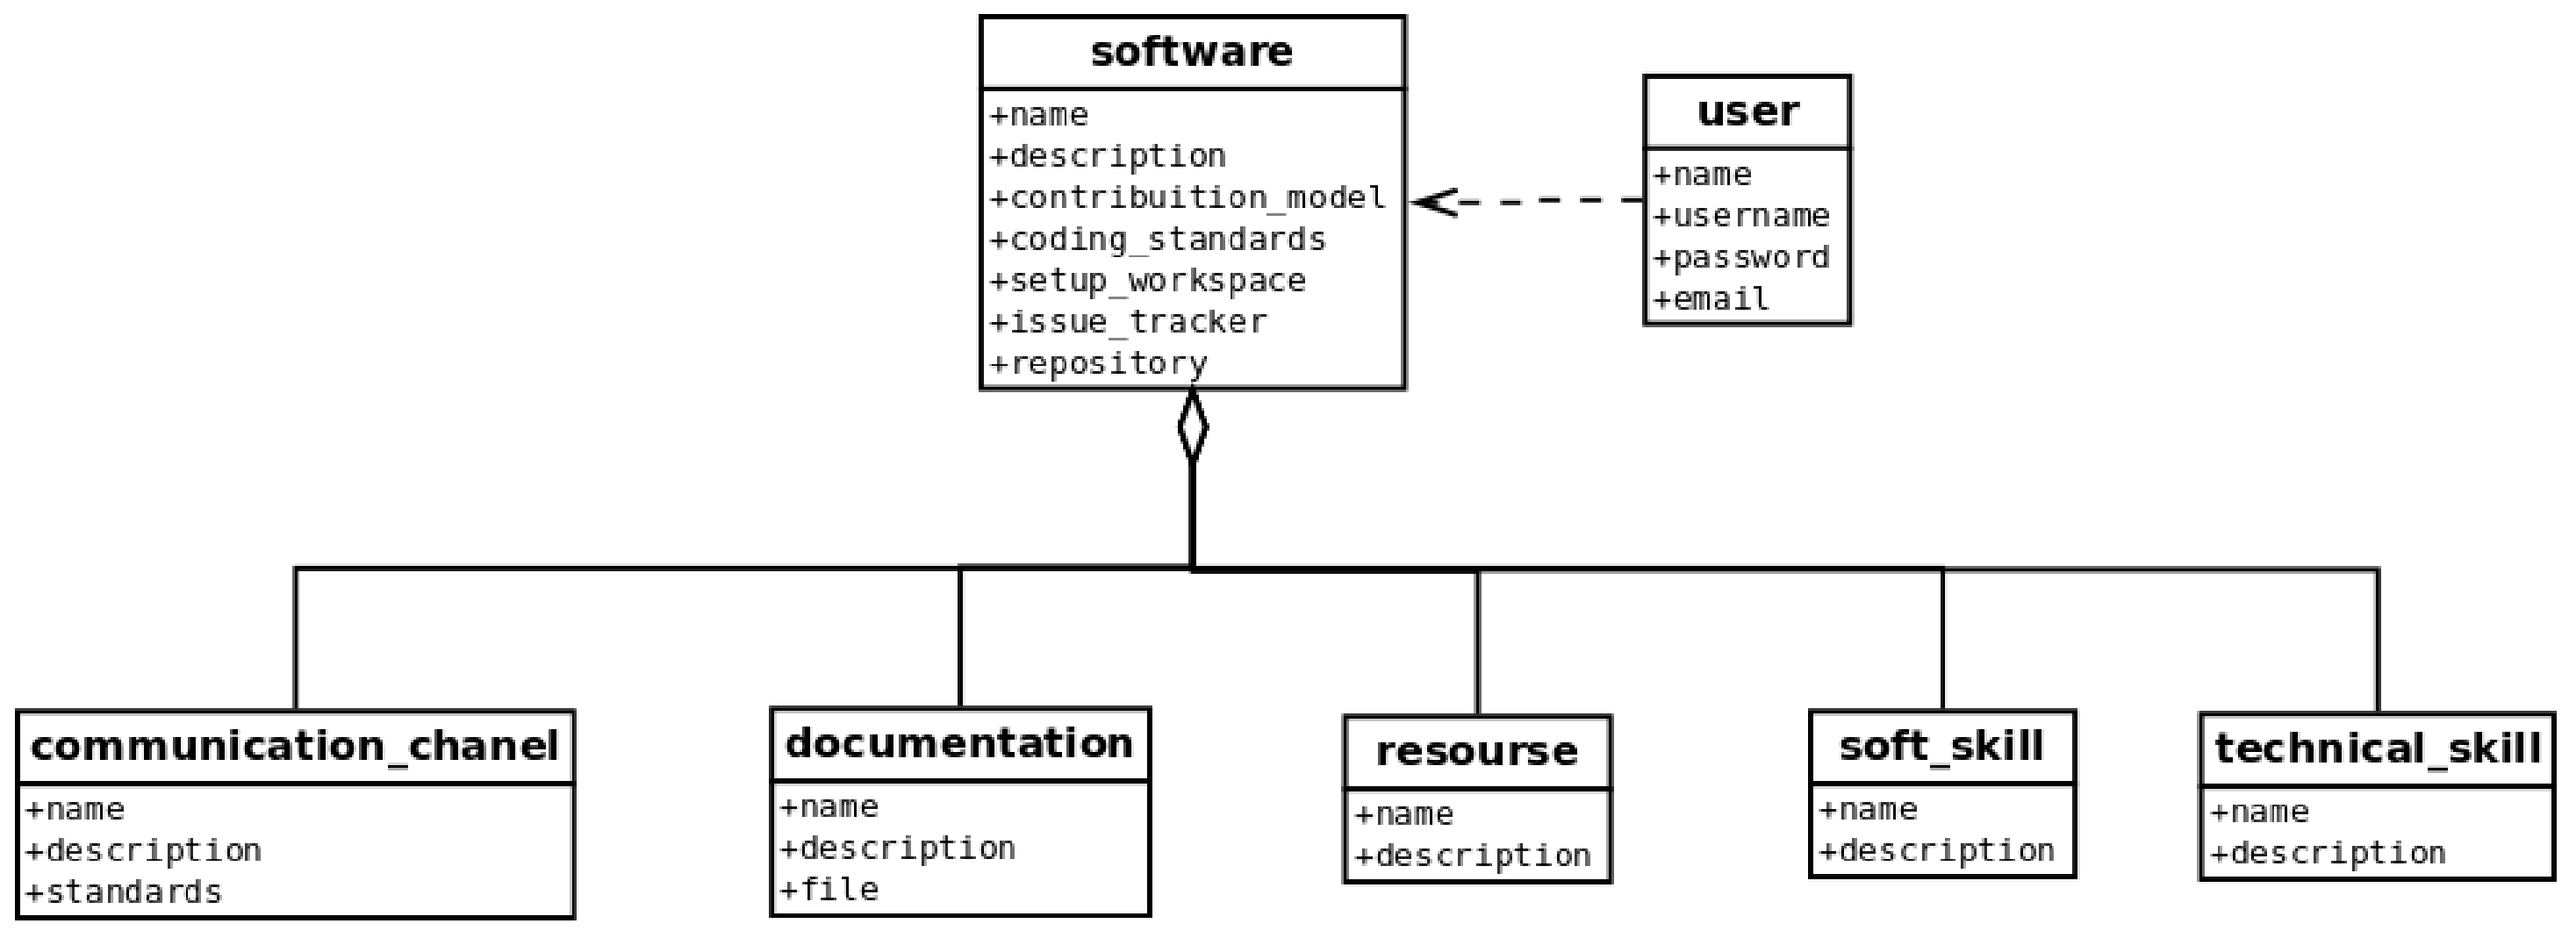
\includegraphics[keepaspectratio=true,scale=0.2]{figuras/diagrama_inicial.eps}
	\caption{Diagrama de dados inicial do novo Portal FlossCoach.}
\end{figure}
}

\frame{
\frametitle{Desenvolvimento do novo Portal FlossCoach}
\begin{figure}[h]
	\centering
	\label{fig:prototipo}
		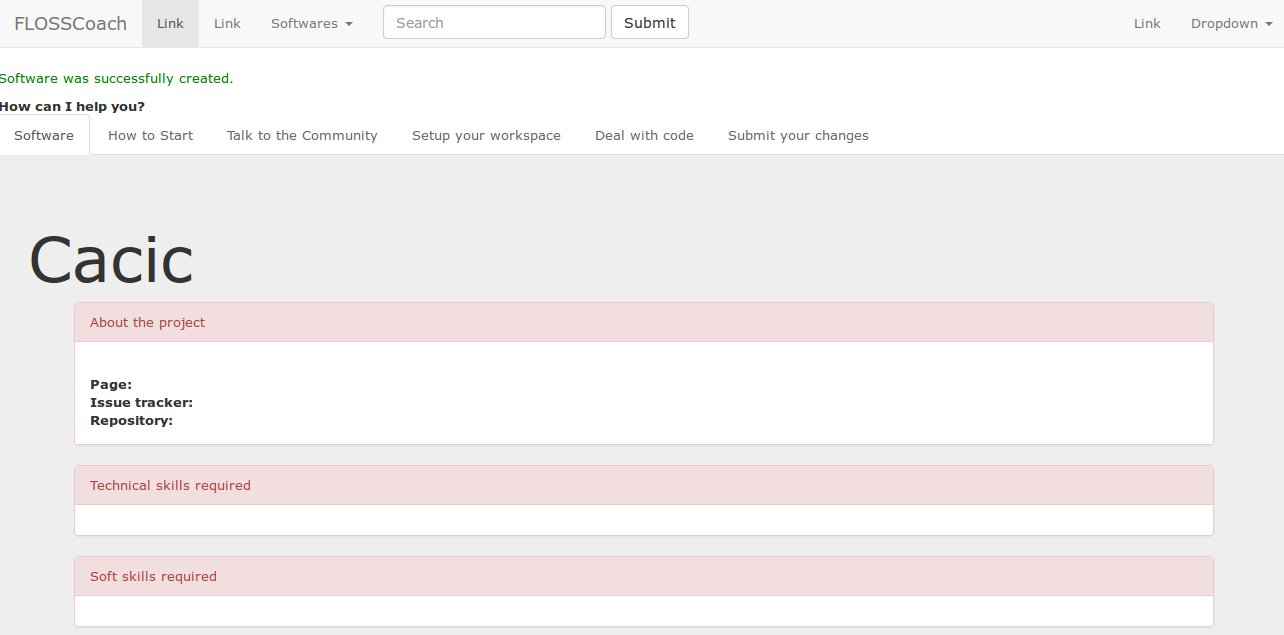
\includegraphics[keepaspectratio=true,scale=0.2]{figuras/prototipo.eps}
	\caption{Prototipo inicial do novo Portal FlossCoach.}
\end{figure}
}

\frame{
\frametitle{Desenvolvimento do novo Portal FlossCoach}
\begin{itemize}
\item Segunda fase do desenvolvimento.
\item Professor Igor Steinmancher montou uma equipe com 2 bolsistas.
\item Passamos a interagir mais frequentemente.
\item Eles implemetaram as modificações que fizeram no diagrama de
dados e melhoraram o front end da aplicação além de desenvolver novas funcionalidades.
\item Esta fase também durou 4 meses, iniciando em abril de 2016 e finalizando em julho de 2016.
\end{itemize}
}

\frame{
\frametitle{Desenvolvimento do novo Portal FlossCoach}
\begin{figure}[h]
	\centering
	\label{fig:diagrama2}
		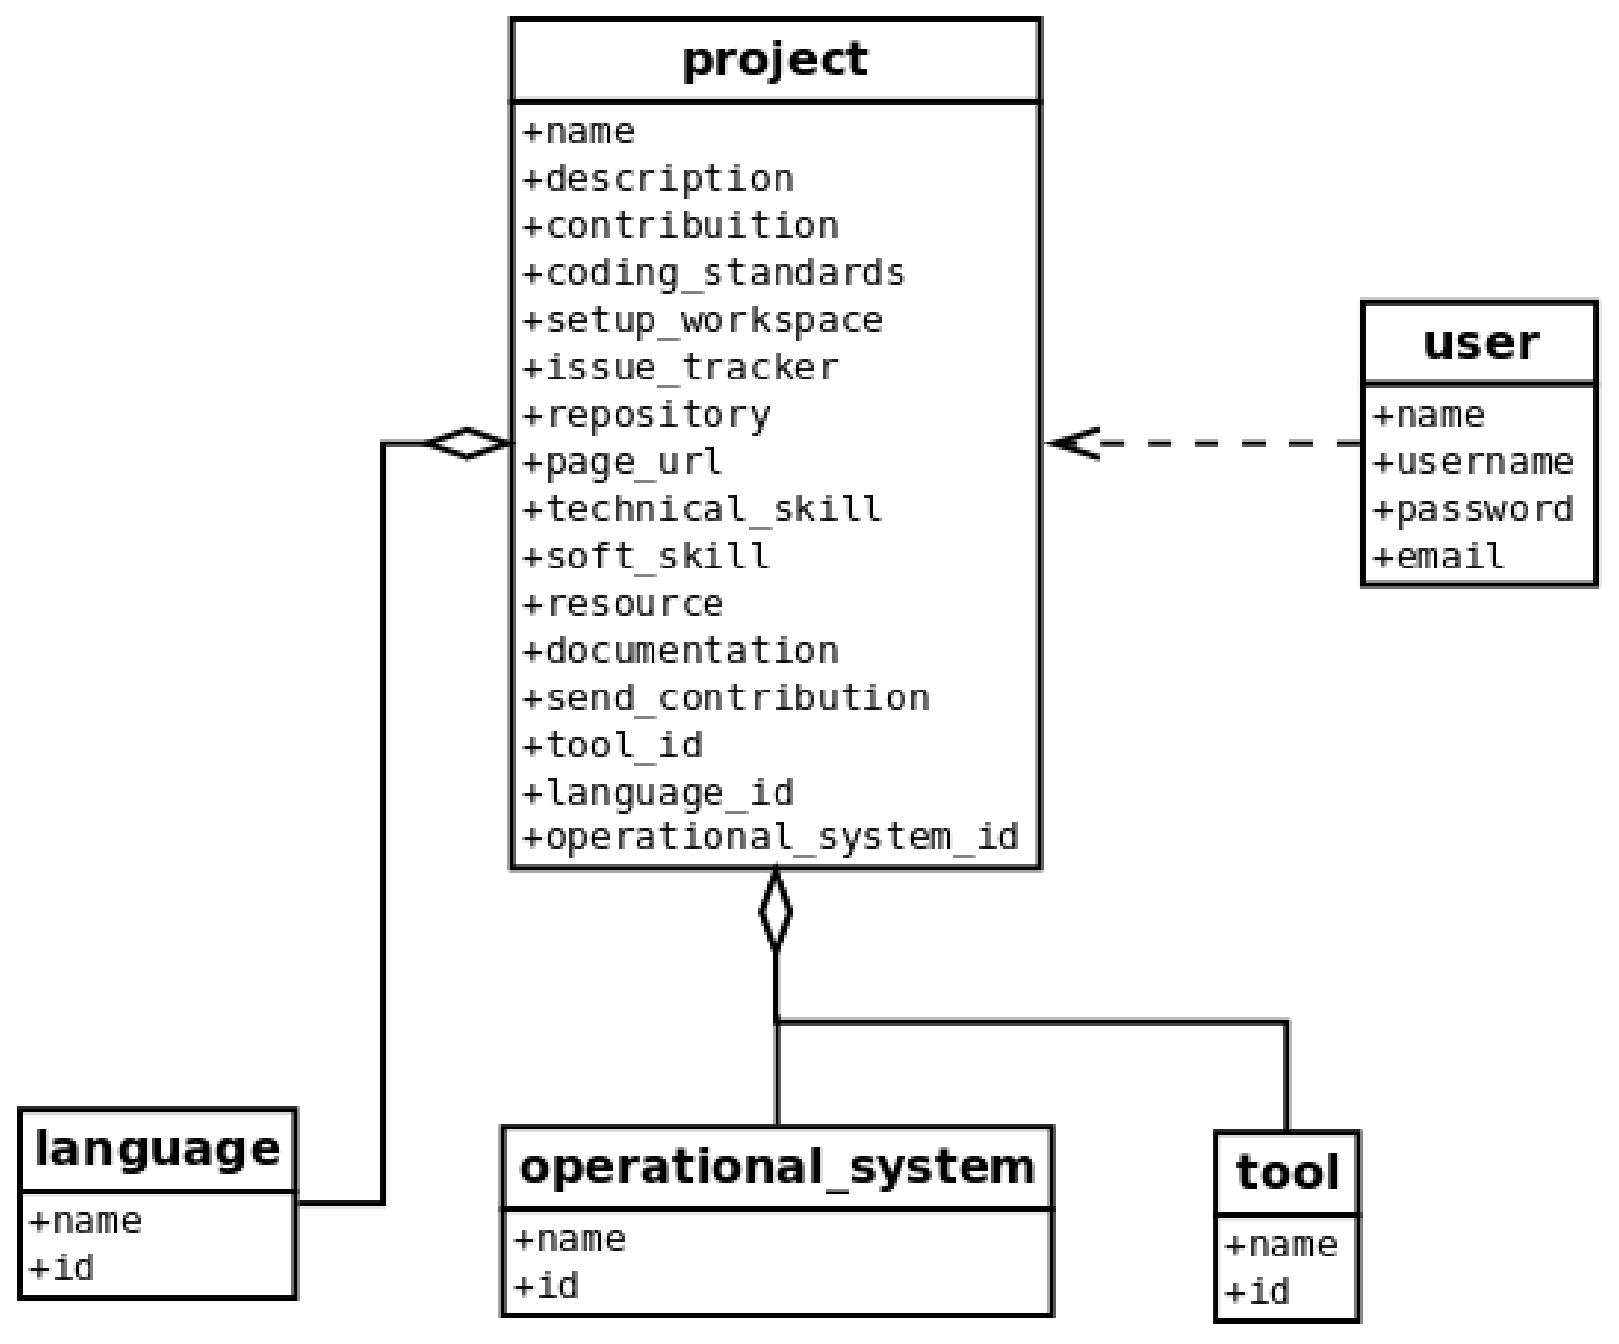
\includegraphics[keepaspectratio=true,scale=0.2]{figuras/diagrama_fase2.eps}
	\caption{Diagrama de dados do novo Portal FlossCoach.}
\end{figure}
}

\frame{
\frametitle{Desenvolvimento do novo Portal FlossCoach}
\begin{figure}[h]
	\centering
	\label{fig:login}
		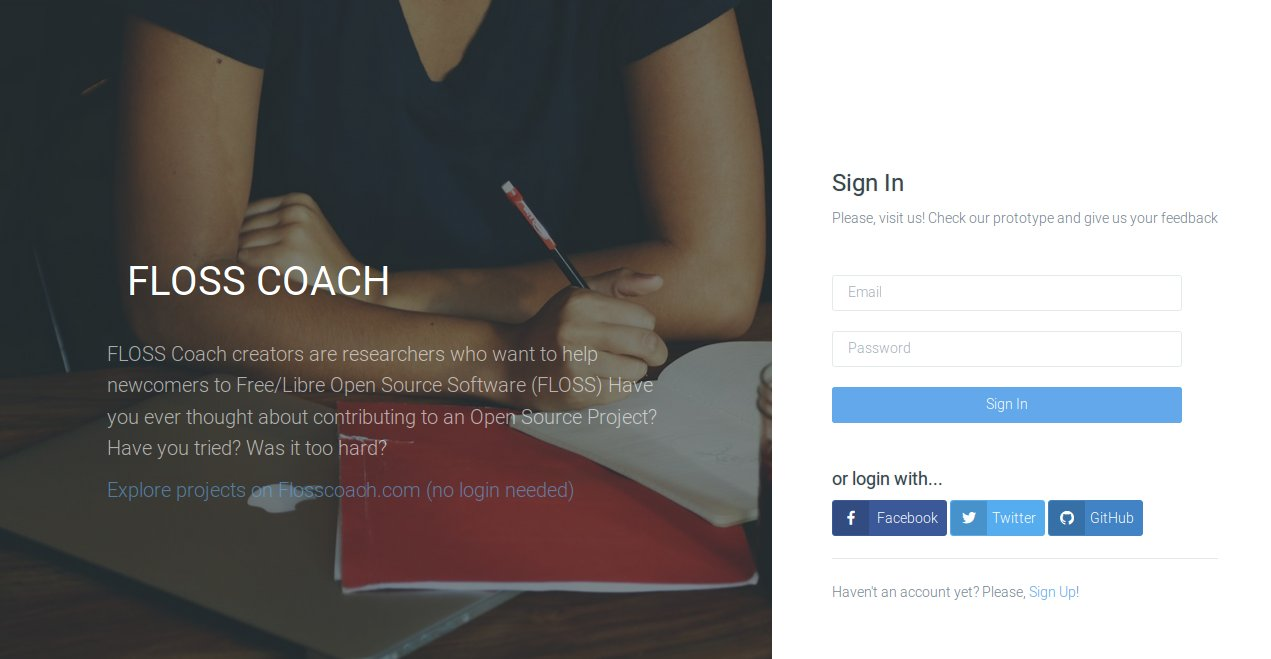
\includegraphics[keepaspectratio=true,scale=0.2]{figuras/login.eps}
	\caption{Página de login do novo Portal FlossCoach.}
\end{figure}
}

\frame{
\frametitle{Desenvolvimento do novo Portal FlossCoach}
\begin{figure}[h]
	\centering
	\label{fig:layout}
		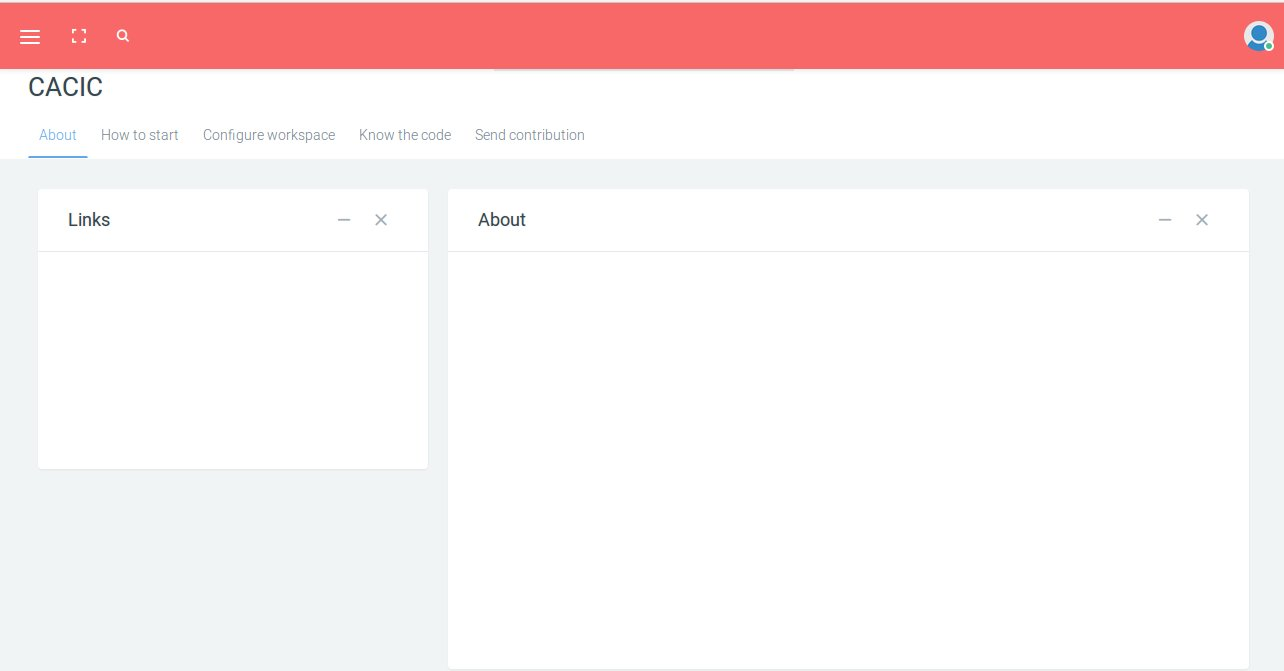
\includegraphics[keepaspectratio=true,scale=0.2]{figuras/layout.eps}
	\caption{Layout do novo Portal FlossCoach após a segunda fase de desenvolvimento.}
\end{figure}
}

\frame{
\frametitle{Desenvolvimento do novo Portal FlossCoach}
\begin{itemize}
\item Terceira fase do desenvolvimento.
\item Projeto entrou na disciplina de Manutenção e Evolução de Software.
\item Equipe de 6 alunos ficou com FlossCoach para desenvolvimento. 
\item A disciplina foi dividida em 6 sprints. 
\end{itemize}
\begin{figure}[h]
	\centering
	\label{fig:sprints}
		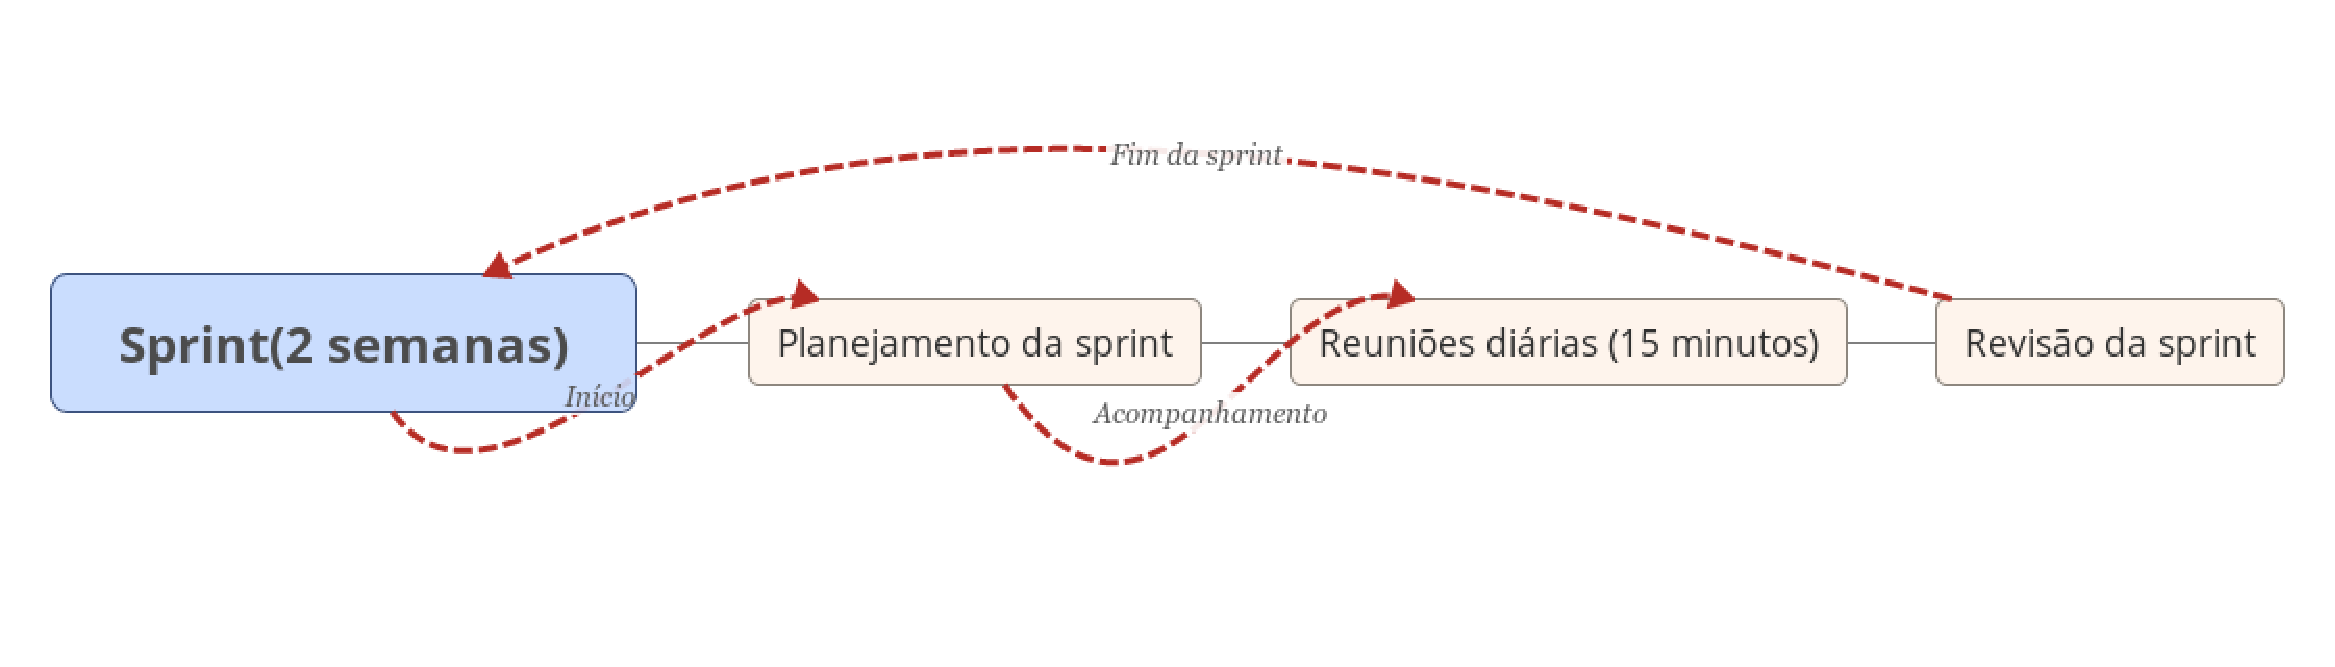
\includegraphics[keepaspectratio=true,scale=0.2]{figuras/Sprint.eps}
	\caption{Dinâmica do desenvolvimento dentro da disciplina.}
\end{figure}
}

\frame{
\frametitle{Desenvolvimento do novo Portal FlossCoach}
\begin{itemize}
\item Ao final da terceira fase o antigo portal FlossCoach foi substituído pela nova versão.
\item na nova versão é possível:
	\begin{itemize}
	\item Cadastrar e editar usuários;
	\item Fazer login através das redes sociais \textit{Facebook}, \textit{Twitter} além do \textit{Github};
	\item Cadastrar e editar projetos;
	\item Buscar informações dos projetos no \textit{OpenHub};
	\item O portal pode ser visto em inglês e português;
	\item Resgatar a senha de usuário.
	\end{itemize}
\end{itemize}
}

\frame{
\frametitle{Desenvolvimento do novo Portal FlossCoach}
\begin{figure}[h]
	\centering
	\label{fig:producao}
		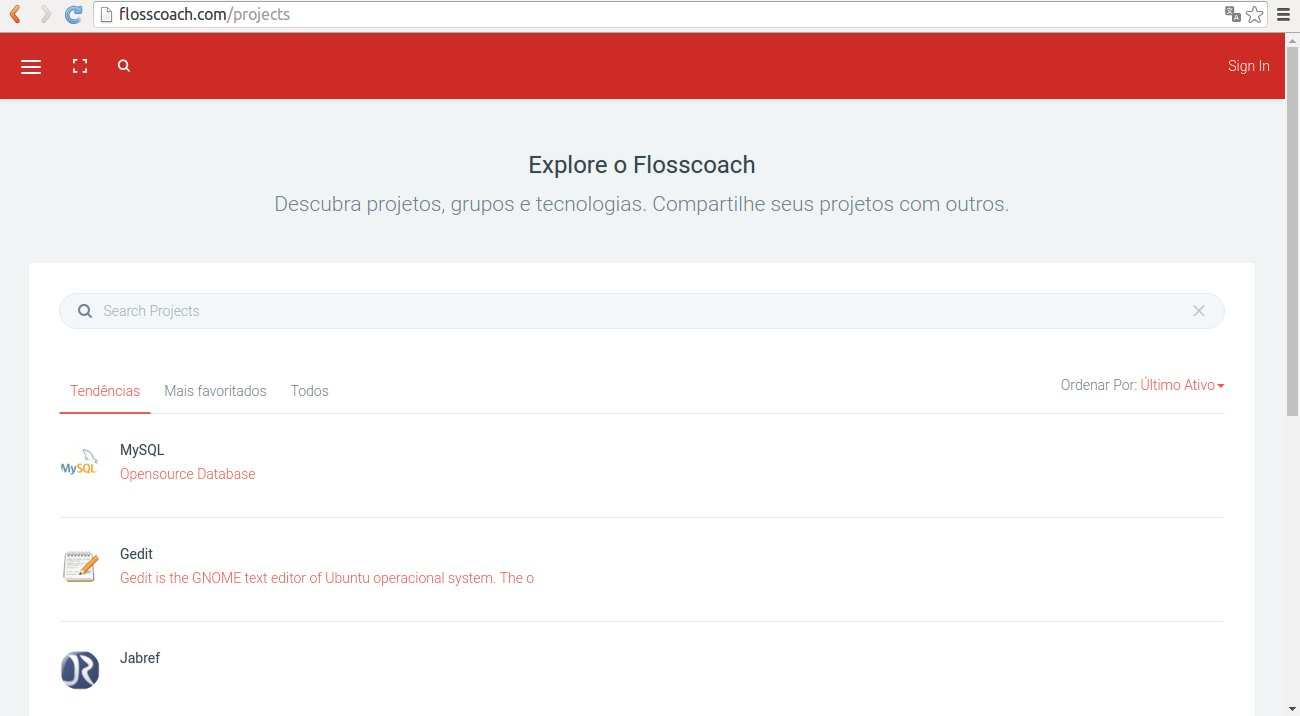
\includegraphics[keepaspectratio=true,scale=0.2]{figuras/flosscoachProducao.eps}
	\caption{Página de projetos do novo Portal FlossCoach}
\end{figure}
}

\frame{
\frametitle{Desenvolvimento do novo Portal FlossCoach}
\begin{figure}[h]
	\centering
	\label{fig:projeto}
		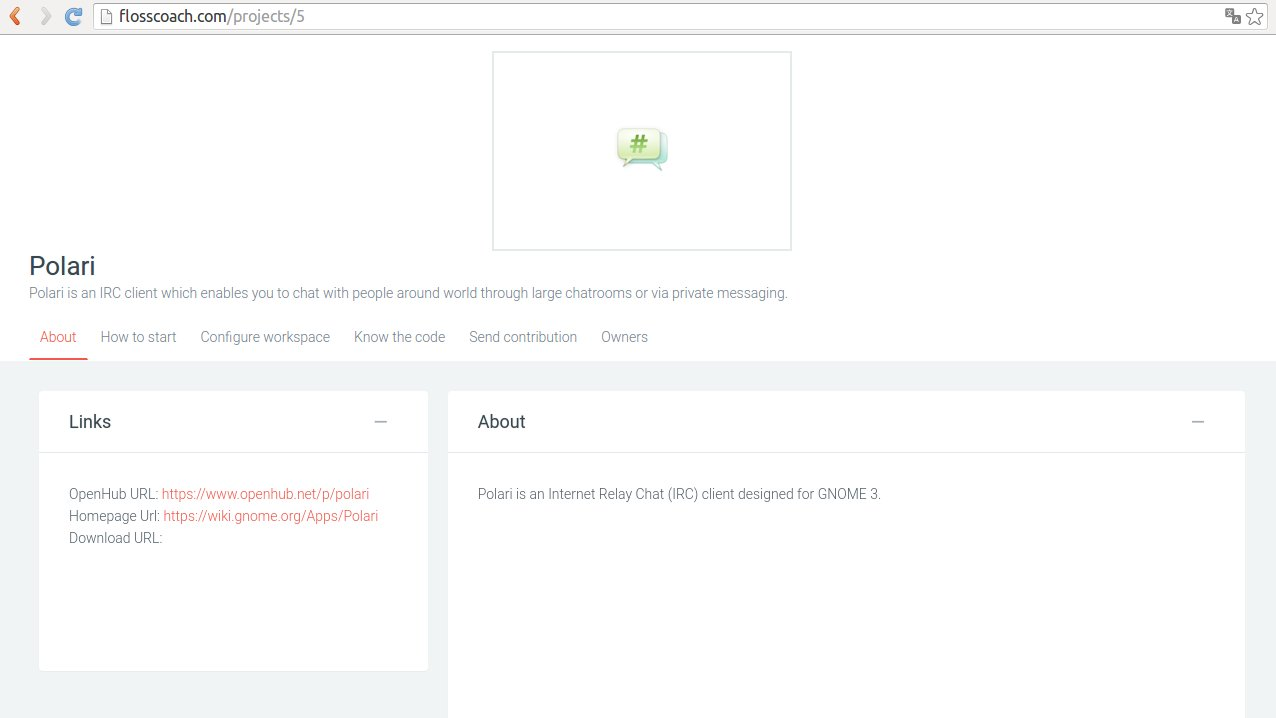
\includegraphics[keepaspectratio=true,scale=0.2]{figuras/paginaprojeto.eps}
	\caption{Página do projeto Polari no novo Portal FlossCoach}
\end{figure}
}

\section{Conclusão}

\frame{
\frametitle{Conclusão}
\begin{itemize}
\item Projetos de software público possuem características que dificultam ainda mais a
entrada de novos desenvolvedores.
\item Os desenvolvedores não sabem diferenciar projetos de software público de projetos de 
software livre.
\item A hierarquia dentro dos órgãos também dificulta o processo de entrada nos projetos.
\end{itemize}
}

\frame{
\frametitle{Conclusão}
\begin{itemize}
\item Os objetivos traçados para esse trabalho foram alcançados.
	\begin{itemize}
	\item Mapeamos através dos questionários as barreiras para contribuir com projetos de software público;
	\item Comparamos as barreiras encontradas com as barreiras para contribuir com projetos de software livre;
	\item Iniciamos o desenvolvimento do novo Portal FlossCoach e a formatação de sua comunidade.
	\end{itemize}
\end{itemize}
}

\frame{
\frametitle{Conclusão}
Respondendo a nossa questão de pesquisa.
\begin{block}{Questão de Pesquisa}
Existem mais barreiras para começar a contribuir com um projeto de software
público do que com um projeto de software livre?
\end{block}
Sim, temos ainda mais barreiras específicas para contribuir com projetos de software público.
\begin{itemize}
\item Falta de conhecimento dos desenvolvedores dos projetos em software livre e público;
\item Rígida hierarquia nos órgãos do governo.
\end{itemize}
}

\frame{
\frametitle{Trabalhos Futuros}
\begin{itemize}
\item Criação de uma nova instância do FlossCoach para atender apenas projetos de software público.
\item Utilizar a API do Noosfero do SPB para buscar informações dos projetos dinamicamente.
\end{itemize}
}

\frame{
Obrigada!
}
\end{document}
